\chapter{Phương thức chia dữ liệu}

% ==========================================
% SECTION 1: K-FOLD CROSS VALIDATION
% ==========================================
\section{K-Fold Cross Validation}

\begin{figure}[H]
    \centering
    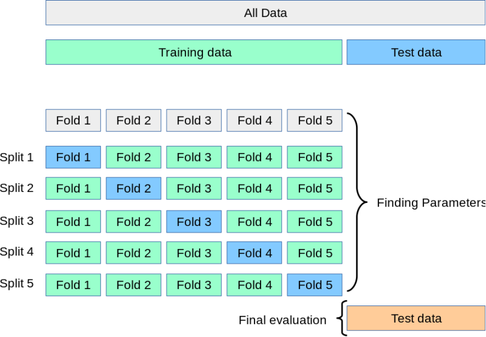
\includegraphics[width=0.8\linewidth]{51.png}
    %\fbox{\parbox[c][4cm][c]{0.8\linewidth}{\centering \textit{[Chèn ảnh: Minh họa K-Fold Cross Validation tại đây]}}}
    \caption{Cơ chế phân chia dữ liệu trong K-Fold Cross Validation}
    \label{fig:kfold_cv}
\end{figure}

\begin{itemize}
    \item \textbf{Mục đích:} Cách chia và tận dụng toàn bộ dữ liệu huấn luyện để đánh giá mô hình một cách khách quan và toàn diện hơn.
    \item \textbf{Test set:} Được tách riêng ra khỏi bộ dữ liệu ban đầu (\textit{unseen data} — không tham gia vào quá trình huấn luyện).
    \item \textbf{Quá trình huấn luyện:} Phần dữ liệu train được chia thành $K$ phần (folds) bằng nhau và thực hiện huấn luyện mô hình $K$ lần. Ở mỗi lần chạy:
    \begin{itemize}
        \item Chọn $1$ phần làm tập \textbf{Validation}.
        \item Chọn $K - 1$ phần còn lại làm tập \textbf{Train}.
    \end{itemize}
    \item \textbf{Đánh giá cuối cùng:} Kết quả đánh giá mô hình là \textbf{trung bình cộng} của tất cả các kết quả thu được sau $K$ lần huấn luyện.
\end{itemize}